\documentclass[aspectratio=169]{beamer}

\usepackage[utf8]{inputenc}
\mode<presentation>
{
  \usetheme{Darmstadt}      % or try Darmstadt, Madrid, Warsaw, ...
  \usecolortheme{beaver} % or try albatross, beaver, crane, ...
  \usefonttheme{serif}  % or try serif, structurebold, ...
  \setbeamertemplate{navigation symbols}{}
  \setbeamertemplate{caption}[numbered]
  \setbeamertemplate{footline}[frame number]
  \setbeamertemplate{headline}{}
} 
\usepackage{graphicx}
\usepackage[english]{babel}
\usepackage[utf8]{inputenc}
\usepackage[T1]{fontenc}
\usepackage{bm}
\usepackage{amssymb}
\usepackage{amsmath}
\usepackage{bm}
\usepackage{leftidx}
\usepackage{mathtools}
\usepackage{tikz}
\usepackage{gensymb}
\usepackage{listings}
\pdfsuppresswarningpagegroup=1

\begin{document}
\AtBeginSection[]{
  \begin{frame}
  \vfill
  \centering
  \begin{beamercolorbox}[sep=8pt,center,shadow=true,rounded=true]{title}
    \usebeamerfont{title}\insertsectionhead\par%
  \end{beamercolorbox}
  \vfill
  \end{frame}
}

\begin{frame}{Aircraft Dynamics}
    \begin{itemize}
        \item State
        \begin{equation*}
            \mathbf{x} = \begin{bmatrix}
                \mathbf{v}_B^T &
                \mathbf{r}_I^T &
                \boldsymbol{\omega}_B^T &
                \boldsymbol{\Theta}^T
            \end{bmatrix}^T
        \end{equation*}
        \item $I$ is the inertial frame; $B$ is the body frame
        \item Kinematics
        \begin{equation*}
            \dot{\mathbf{r}}_I = \mathbf{H}_B^I \mathbf{v}_I \qquad
            \dot{\boldsymbol{\Theta}} = \mathbf{L}_B^E \boldsymbol{\omega}_B
        \end{equation*}
        \item Overall dynamics
        \begin{equation*}
            \dot{\mathbf{x}} = \mathbf{f}(\mathbf{x},\mathbf{u},t)
        \end{equation*}
    \end{itemize}
\end{frame}

\begin{frame}{Sliding Surface for Aircraft Control}
    \begin{itemize}
        \item We want the aircraft to follow a specified state $\mathbf{r}^*_I(t)$, $\boldsymbol{\Theta}^*(t)$
        \item We want to confine the aircraft's motion to the hypersurface on which
        \begin{equation*}
            \delta \dot{\mathbf{r}}_I= -K_r \delta \mathbf{r}_I \qquad \delta \dot{\boldsymbol{\Theta}} = -K_\theta \delta \boldsymbol{\Theta}
        \end{equation*}
        where
        \begin{equation*}
            \delta \mathbf{r}_I = \mathbf{r}_I - \mathbf{r}_I^* \qquad \delta \boldsymbol{\Theta} = \boldsymbol{\Theta}-\boldsymbol{\Theta}^*
        \end{equation*}
        \item Combined with kinematics, this defines our ``sliding surface''
        \begin{equation*}
            \boldsymbol{\sigma}(\mathbf{x}) = 
            \begin{bmatrix}
                \mathbf{H}_B^I \mathbf{v}_I - \dot{\mathbf{r}}_I^* + K_r ( \mathbf{r}_I - \mathbf{r}_I^*) \\
                \mathbf{L}_B^E \boldsymbol{\omega}_B - \dot{\boldsymbol{\Theta}}^* + K_\theta(\boldsymbol{\Theta}-\boldsymbol{\Theta}^*) 
            \end{bmatrix} = \mathbf{0}
        \end{equation*}
        \item Aircraft state is exponentially stable on sliding surface
    \end{itemize}
\end{frame}

\begin{frame}{Sliding Surface for Aircraft Control}
    \begin{itemize}
        \item Sliding surface can be expressed as
        \begin{equation*}
            \boldsymbol{\sigma} = \mathbf{S}\mathbf{x} - \mathbf{S}^*\mathbf{x}^* = \mathbf{0}
        \end{equation*}
        where
        \begin{equation*}
            \mathbf{S}(\mathbf{x}) = \begin{bmatrix}
                \mathbf{H}_B^I & K_r\mathbf{I} & \mathbf{0} & \mathbf{0} \\
                \mathbf{0} & \mathbf{0} & \mathbf{L}_B^E & K_\theta\mathbf{I}
            \end{bmatrix}
        \end{equation*}
        \item Then
        \begin{equation*}
            \dot{\boldsymbol{\sigma}} = \dot{\mathbf{S}}\mathbf{x} + \mathbf{S}\dot{\mathbf{x}} - \dot{\mathbf{S}}^*\mathbf{x}^* - \mathbf{S}\dot{\mathbf{x}}^*
        \end{equation*}
    \end{itemize}
\end{frame}

\begin{frame}{Aircraft Sliding Mode Control}
    \begin{itemize}
        \item Linearize dynamics with respect to controls $\mathbf{u}$
        \begin{equation*}
            \dot{\mathbf{x}} = \mathbf{f}(\mathbf{x},\mathbf{u},t) = \mathbf{h}(\mathbf{x},\mathbf{u},t) + \mathbf{B} (\mathbf{u} - \mathbf{u}^*)
        \end{equation*}
        \item Substitute into sliding mode derivative
        \begin{equation*}
            \dot{\boldsymbol{\sigma}} = \dot{\mathbf{S}}\mathbf{x} + \mathbf{S}[\mathbf{h}(\mathbf{x},\mathbf{u},t) + \mathbf{B} (\mathbf{u} - \mathbf{u}^*)] - \dot{\mathbf{S}}^*\mathbf{x}^* - \mathbf{S}\dot{\mathbf{x}}^*
        \end{equation*}
    \end{itemize}
\end{frame}

\begin{frame}{Aircraft Sliding Mode Control}
    \begin{itemize}
      \item Choose a constant $L$ such that
        \begin{equation*}
            |\{\dot{\mathbf{S}}\mathbf{x} - \mathbf{S}\mathbf{h}(\mathbf{x},\mathbf{u},t) - \dot{\mathbf{S}}^*\mathbf{x}^* - \mathbf{S}\dot{\mathbf{x}}^*\}_i| < L
        \end{equation*}
        \item Then if $\mathbf{S}\mathbf{B} (\mathbf{u} - \mathbf{u}^*) = -L \mathrm{sgn}(\boldsymbol{\sigma})$,
        \begin{equation*}
            \frac{d}{dt}\left(\frac{1}{2}\boldsymbol{\sigma}^T\boldsymbol{\sigma}\right) = \boldsymbol{\sigma}^T\dot{\boldsymbol{\sigma}} < 0
        \end{equation*}
        so the system reaches $\boldsymbol{\sigma}=\mathbf{0}$ in finite time
    \item Finally, we obtain the control
    \begin{equation*}
        \mathbf{u} = \mathbf{u}^* -L (\mathbf{S}\mathbf{B})^{-1} \mathrm{sgn}(\boldsymbol{\sigma})
    \end{equation*}
        \item In practice, use sigmoid instead of sgn to avoid ``chatter''
        \end{itemize}
\end{frame}

\begin{frame}{Through the Hurricane}
    \centering
    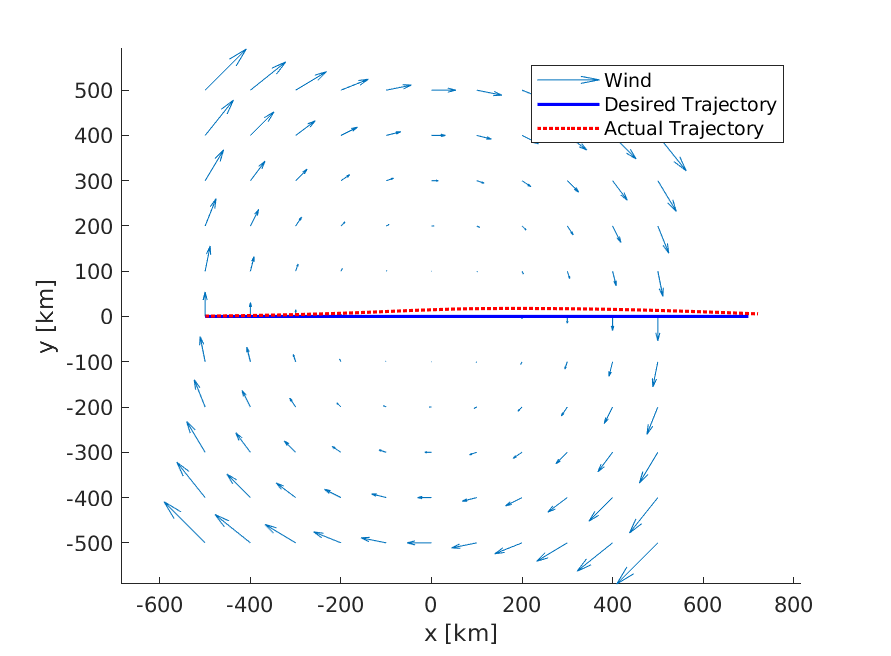
\includegraphics[width=0.49\textwidth]{sm_hurricane.png} 
    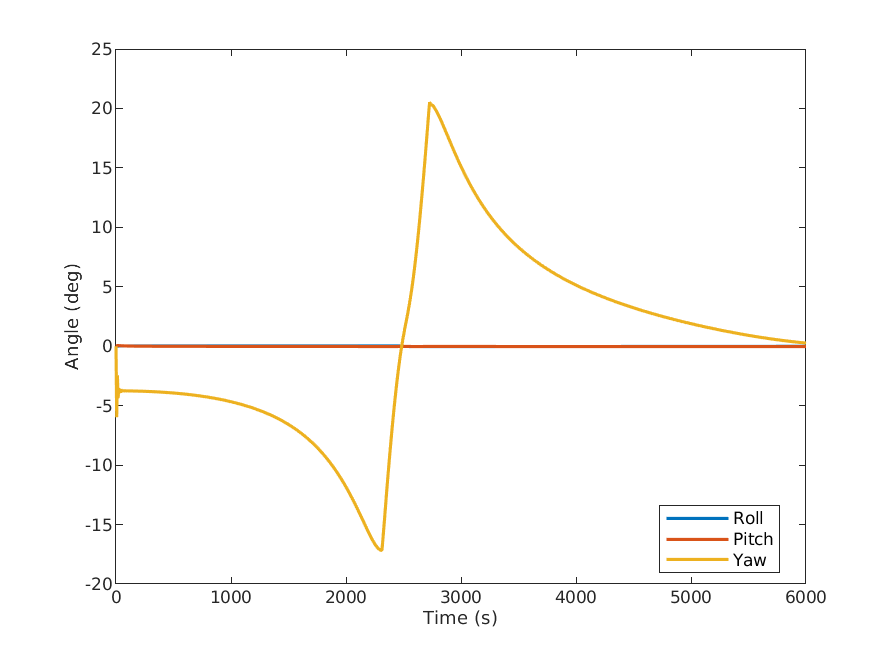
\includegraphics[width=0.49\textwidth]{sm_rpy.png}
\end{frame}

\end{document}

\begin{frame}{Introduction to Sliding Mode Control}
    \begin{itemize}
        \item For a dynamical system with state $\mathbf{x}$, choose a ``sliding surface'' $\boldsymbol{\sigma}(\mathbf{x})=\mathbf{0}$
        \item State must be stable on this surface
        \begin{itemize}
            \item For example, if $\mathbf{x}=\begin{bmatrix}
                x & \dot{x}
            \end{bmatrix}^T$, we can set $\sigma(\mathbf{x})=\dot{x}+kx$
        \end{itemize}
    \end{itemize}
\end{frame}